\documentclass[11pt]{article}
\usepackage[margin=1.15in]{geometry}
\usepackage{amsmath,amssymb,amsthm}
\usepackage{booktabs}
\usepackage{graphicx}
\usepackage{microtype}
\usepackage[authoryear,round]{natbib}
\usepackage[colorlinks=true,linkcolor=black,citecolor=black,urlcolor=black]{hyperref}
\usepackage{setspace}
\onehalfspacing

\newtheorem{proposition}{Proposition}
\theoremstyle{definition}
\newtheorem{definition}{Definition}

\newcommand{\E}{\mathbb{E}}
\newcommand{\Var}{\operatorname{Var}}

\title{Overlapping Error Bars Prove Nothing\\[4pt]
\large Paired Inference and the Unit of Replication}
\author{Flyxion\\Independent Researcher}
\date{October 2026}

\begin{document}
\maketitle

\begin{abstract}
\noindent
Two practices in the reading of benchmark tables are common enough to pass as method. The first treats overlapping error bars as evidence that two methods do not differ. The second treats a significance test with a very small $P$ value as evidence that one method is better than the other. Both rest on a misidentification of what the interval or the test is about. The first confuses the uncertainty of each estimate with the uncertainty of their difference, which can be far smaller when the methods are evaluated on the same items. The second confuses the population over which the test varies, usually the test items, with the population over which a claim about a method must hold, which includes training runs. This essay derives what the overlap rule actually tests, shows that its effective size collapses as the correlation between methods grows, and shows that a paired test over test items has a variance floor set by training-run variability that no number of test items removes. Simulations with 200 shared scenes and with up to 20{,}000 test items illustrate each result. A recent perturbation-modeling paper that tests models against baselines with comparisons paired by perturbation is used as a worked example of what a correctly paired design does and does not cover. The conclusions concern inference and do not evaluate any particular benchmark.
\end{abstract}

\section{Two rules of thumb}

A table lists a score for each of several methods, each with an interval. A reader checks whether the intervals of two methods overlap. If they do, the reader concludes that the methods are not distinguishable, and the difference in the point estimates is attributed to noise. In the opposite situation, a paper reports that a new method beats a baseline with $P<10^{-10}$, and the reader concludes that the new method is better.

Both inferences are reasonable in some designs and badly wrong in others, and the designs in which they fail are the common ones in machine learning evaluation, where methods are scored on the same test items. This essay explains why, using quantities that can be computed exactly.

The argument has two parts. The first concerns what the overlap of two intervals tells a reader about their difference. It is little, and in paired designs it is close to nothing. The second concerns what a paired test establishes. It establishes a statement about the particular trained models over the population of test items. It does not establish a statement about the method, whose behavior also varies across training runs. The first part warns against reading too little into overlap. The second warns against reading too much into a small $P$ value.

\section{What an interval is an interval for}

An error bar is a summary of variation, and the first question about it is which variation. Three quantities are plotted under the same visual convention. The standard deviation describes how scores vary across the items in the sample. The standard error of the mean describes how a mean computed from that many items would vary across repeated samples of items. A confidence interval is built from the standard error and a reference distribution. A plot that does not say which was drawn cannot be read, and bars that overlap in standard deviation say nothing about the means, since the standard deviation does not shrink with the number of items.

The second question is which source of variation is resampled. A benchmark score depends on the test items, on the random initialization and data order of each training run, on any stochasticity at inference, and on the training data. An interval that resamples items describes uncertainty about the score of these trained models on a population of items. An interval that resamples training runs describes uncertainty about the score a freshly trained model would obtain. The two answer different questions, and an interval of one kind is silent about the other. Sections 3 to 5 concern the first source, and Section~6 concerns the second.

\section{The overlap rule as a test}

Let two methods have estimated scores $\hat m_A$ and $\hat m_B$ with standard errors $s_A$ and $s_B$ and normal $95\%$ intervals $\hat m\pm1.96\,s$. The intervals fail to overlap exactly when $|\hat m_A-\hat m_B|>1.96\,(s_A+s_B)$. A standard test of the difference, when the estimates are independent, rejects at the $5\%$ level when $|\hat m_A-\hat m_B|>1.96\sqrt{s_A^2+s_B^2}$. Since $s_A+s_B\ge\sqrt{s_A^2+s_B^2}$, non-overlap implies significance, but not conversely, and the gap can be large.

\begin{proposition}
Suppose $s_A=s_B=s$ and the estimates are independent and normal. The difference is significant at the $5\%$ level when $|\hat m_A-\hat m_B|>2.77\,s$, whereas the intervals separate only when $|\hat m_A-\hat m_B|>3.92\,s$. A decision rule that declares a difference only when the intervals do not overlap is a test of size $2\bar\Phi(3.92/\sqrt2)\approx0.0056$, not $0.05$.
\end{proposition}

\begin{proof}
Under the null the difference has standard error $\sqrt2\,s$, so $P(|\hat m_A-\hat m_B|>3.92\,s)=P(|Z|>3.92/\sqrt2)=P(|Z|>2.77)=0.0056$. \qedhere
\end{proof}

The rule is therefore conservative. It was not designed as a test, and nothing is wrong with a conservative test, but a reader who treats overlap as ``not significantly different at the $5\%$ level'' has attributed to the rule a property it does not have. The range of differences between $2.77\,s$ and $3.92\,s$ is significant at $5\%$ while the intervals overlap.

This is the situation with independent estimates. The situation with paired estimates is worse for the rule. Suppose the two methods are evaluated on the same items, and their per-item scores have correlation $\rho$. The standard error of the difference of the means is $s\sqrt{2(1-\rho)}$, not $s\sqrt2$, because the variation shared by the two methods cancels in the difference but remains in each interval. The intervals do not narrow with $\rho$. The rule's implied threshold, expressed in standard errors of the difference, is therefore $3.92/\sqrt{2(1-\rho)}$ and its size is $2\bar\Phi$ of that.

\begin{table}[t]
\centering
\caption{Effective size of the non-overlap rule when the two methods are scored on the same items with per-item correlation $\rho$, normal approximation, equal standard errors. The paired $t$ test has size $0.05$ at every $\rho$.}
\begin{tabular}{rcc}
\toprule
$\rho$ & threshold in SEs of the difference & size of the non-overlap rule \\
\midrule
0.00 & 2.77  & $5.6\times10^{-3}$ \\
0.50 & 3.92  & $8.9\times10^{-5}$ \\
0.80 & 6.20  & $5.7\times10^{-10}$ \\
0.95 & 12.40 & $<10^{-34}$ \\
\bottomrule
\end{tabular}
\end{table}

Table~1 gives the consequence. At $\rho=0.8$ the rule would call two methods different only when the observed difference exceeds six standard errors, which for a true effect exactly at the test's threshold is a power of nearly zero. Correlations of this size are not exotic when the items vary much in difficulty and every method finds the hard items hard, which is the usual case in benchmarks built from scenes, images or questions. The per-item correlation between two methods is rarely reported, and it is the quantity that decides how misleading overlap is.

\section{A simulation with shared items}

The simulation uses $N=200$ items. Each item has a difficulty $s_i\sim N(0,\tau^2)$ shared by both methods, and each method's score on the item is its mean plus $s_i$ plus independent noise of standard deviation one. The true difference between the methods is $d$. The per-item correlation is $\rho=\tau^2/(\tau^2+1)$. Three decision rules are applied: the non-overlap of two $95\%$ $t$ intervals for the means, an unpaired Welch test, and a paired $t$ test. Each row averages 4000 simulated benchmarks.

\begin{table}[t]
\centering
\caption{Rejection rates of three rules at $N=200$ shared items with true difference $d=0$ (size) and $d=0.4$ (power). The half-width is that of each method's own $95\%$ interval.}
\begin{tabular}{rrccccccc}
\toprule
$\tau$ & $\rho$ & half-width & \multicolumn{2}{c}{non-overlap} & \multicolumn{2}{c}{unpaired $t$} & \multicolumn{2}{c}{paired $t$} \\
 & & & $d=0$ & $d=0.4$ & $d=0$ & $d=0.4$ & $d=0$ & $d=0.4$ \\
\midrule
0 & 0.00 & 0.139 & 0.003 & 0.889 & 0.052 & 0.981 & 0.050 & 0.978 \\
1 & 0.50 & 0.197 & 0.000 & 0.526 & 0.005 & 0.892 & 0.051 & 0.983 \\
2 & 0.80 & 0.311 & 0.000 & 0.015 & 0.000 & 0.362 & 0.046 & 0.980 \\
4 & 0.94 & 0.575 & 0.000 & 0.000 & 0.000 & 0.000 & 0.045 & 0.979 \\
\bottomrule
\end{tabular}
\end{table}

Table~2 shows the structure. The paired test keeps its size and its power of about $0.98$ at every $\tau$, because the shared difficulty cancels in the difference. The marginal intervals widen with $\tau$, since the item-to-item spread grows. At $\tau=2$ each interval has half-width $0.31$, the difference of $0.4$ is smaller than the sum of half-widths $0.62$, the intervals overlap, and the non-overlap rule rejects in $1.5\%$ of simulated benchmarks. The paired test rejects in $98\%$. At $\tau=4$ the non-overlap rule and even the unpaired test have no power, and the paired test is unaffected. The first row, with $\tau=0$ and $\rho=0$, confirms the independent case: the non-overlap rule is conservative, with a size of $0.0054$ in a longer run of 60{,}000 simulated benchmarks, against $0.0056$ from Proposition~1, and the unpaired and paired tests agree.

\begin{figure}[t]
\centering
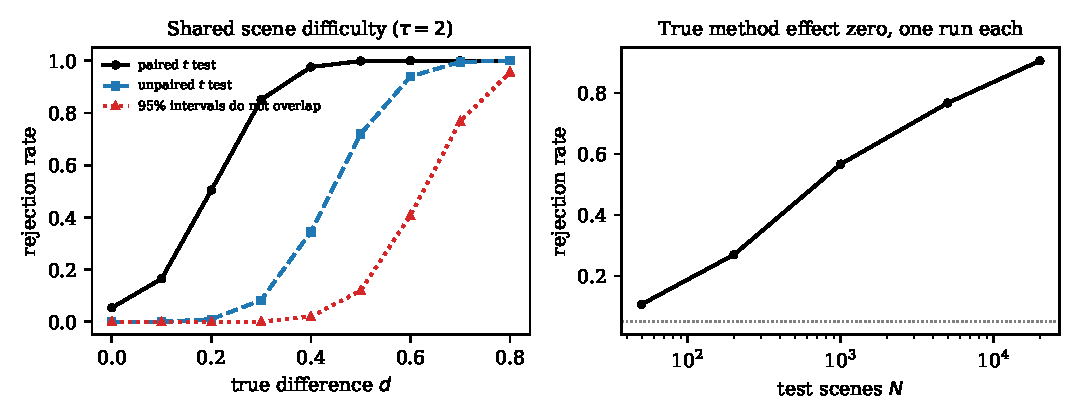
\includegraphics[width=\textwidth]{fig_paired.pdf}
\caption{Left: rejection rate against the true difference at $N=200$ and $\tau=2$ for the paired $t$ test, the unpaired $t$ test, and non-overlap of $95\%$ intervals. Right: rejection rate of a paired test over $N$ shared scenes when the true method effect is zero and each method has one training run (Section~6).}
\end{figure}

The pairing here is the experimental design that makes the gain possible. A paired test uses the cancellation of whatever the two methods share. If the pairing variable does not explain the variance, so that $\rho\le0$, the paired standard error is no smaller than the unpaired one, and the paired test loses a little power for its halved degrees of freedom. The benefit is therefore conditional on the correlation, and the useful report is the correlation, or equivalently the standard deviation of the per-item differences, not only the two marginal intervals.

\section{Not significant is not different}

The converse error runs in the opposite direction. Two methods are each compared with a common baseline. The first improves on it by a margin with $z=2.5$ and the second by one with $z=1$, and a text concludes that the first works and the second does not, and so the first is better. This reading treats the difference in significance as a significant difference \citep{gelman2006}.

Suppose the two improvements are $25\pm10$ and $10\pm10$ in the same units, with independent errors. The first is significant, with $z=2.5$, and the second is not, with $z=1$. Their difference is $15$ with standard error $\sqrt{10^2+10^2}=14.1$, so $z=1.06$, and the data give no basis for saying the two methods differ. The same arithmetic applies to a table that marks entries significant against a baseline with an asterisk. Whether method A is better than method B has to be tested as a difference between A and B, preferably paired, and cannot be read off from the pattern of asterisks.

\section{What pairing does not license}

The paired test of Sections 3 and 4 resamples items. It answers the question: for these two trained models, is the mean score difference over the population of items distinguishable from zero? Training randomness is not varied, so it is silent about whether another run of the training procedure would give the same ordering.

Let each training run $r$ of method $M$ have an offset $\eta_{M,r}$ with standard deviation $\omega$, representing the run-to-run variation in the true score of the trained model. Scoring one run of each method on $N$ shared items gives a paired difference with variance
\[
\Var(\hat d)=\frac{2\sigma_e^2}{N}+2\omega^2,
\]
where $\sigma_e^2$ is the variance of the per-item idiosyncratic noise. The paired test estimates only the first term, so as $N$ grows the test statistic grows without bound, while the quantity that the claim about the method depends on has a floor at $2\omega^2$. The offset $\eta_A-\eta_B$ becomes ``significant'' once $N$ is large enough that the standard error falls below it.

\begin{proposition}
Suppose the true expected scores of methods $A$ and $B$ are equal, and a single run of each is evaluated on $N$ shared items with a paired test. The probability of rejection tends to one as $N\to\infty$ whenever $\omega>0$.
\end{proposition}

\begin{proof}
The test statistic is $(\eta_A-\eta_B+\bar e)/\widehat{\mathrm{SE}}$, where $\bar e$ is the mean of the per-item noise differences, whose standard error vanishes as $N^{-1/2}$. For fixed nonzero $\eta_A-\eta_B$ the numerator converges to it and the denominator to zero. \qedhere
\end{proof}

\begin{table}[t]
\centering
\caption{Paired test rejection rate over $N$ shared items when the true method effect is zero, each method has a single training run with run-to-run standard deviation $\omega=0.1$, $\tau=2$ and idiosyncratic standard deviation one. Nominal level $0.05$.}
\begin{tabular}{rc}
\toprule
$N$ & rejection rate \\
\midrule
50     & 0.11 \\
200    & 0.27 \\
1{,}000  & 0.57 \\
5{,}000  & 0.77 \\
20{,}000 & 0.91 \\
\bottomrule
\end{tabular}
\end{table}

Table~3 shows the consequence. With two methods that are equal in expectation and run-to-run variation of $0.1$, a paired test on $20{,}000$ items rejects the null $91\%$ of the time. The test is correct about what it tests, since the two checkpoints do differ. A conclusion about the method does not follow. More test items buy resolution of the particular checkpoints and nothing about the training procedure.

The remedy is a different design. Train $K$ runs of each method, score each run on the shared items, and compare the two sets of $K$ run-level scores. In the same simulation with $K=5$ runs per method and $N=200$ items, the rejection rate under a zero true effect is $0.046$, close to nominal. With a true difference of $0.1$ the rejection rate is $0.19$, with $0.2$ it is $0.60$, and with $0.3$ it is $0.91$. This design has less power per item than the single-run paired test and tests the right thing. The standard error of the difference is now $\sqrt2\,\omega/\sqrt K$ plus a term that vanishes in $N$, and the floor is correctly part of it. \citet{dietterich1998} treated the related issue of choosing tests for comparing learning algorithms when training-set variation and run variation both matter.

\subsection{A worked example of a correctly paired design}

A recent paper on genetic perturbation models provides a clear instance of a design that is paired where the pairing matters \citep{miller2026}. Its Methods state that hypothesis tests comparing models, baselines and metrics were ``paired by perturbation,'' with each perturbation contributing one summary value per condition, so that the sample size is the number of perturbations. Parametric comparisons use paired Student $t$ tests and nonparametric ones paired Wilcoxon signed-rank tests, with Bonferroni correction across comparisons. The forest plots give $95\%$ intervals for the mean difference obtained by percentile bootstrap over the per-perturbation paired differences, and summary statistics are reported as mean $\pm$ s.e.m.\ across perturbations. Perturbations differ widely in how strong their effects are, so a perturbation-level pairing removes a large shared source of variation, in the manner of Section~4.

What the intervals are intervals for is stated in the same description: they resample perturbations. A reviewer asked, in the first round, exactly the question of Section~2, namely what is resampled in the bootstrap, perturbations or cells, and whether the paired structure is preserved, and the revised Methods answer that the per-perturbation paired differences are resampled with replacement \citep{miller2026peer}. Supplementary Table~2 reports ``mean performance $\pm$ SEM'' for every model and metric with $n$ equal to the number of perturbations per condition (2045, 2323, 238 and 187 across the four tasks), and the Methods describe summary statistics, such as the $0.027\pm0.001$ reported in the main text for the weighted squared error of one model, as mean $\pm$ s.e.m.\ across perturbations unless otherwise indicated \citep{miller2026supp}. Neither the main text, the Methods, the supplementary notes nor the supplementary tables read for this essay describe replicate training runs of each model. Earlier versions of the manuscript specified one-sided paired tests, which a reviewer objected cannot detect underperformance, and the published Methods and figure legends specify paired two-sided tests \citep{miller2026peer}. The statements the design supports are therefore statements about the trained models in the paper over the population of perturbations in each dataset. That is the question the authors set out to answer, namely whether models can outperform uninformative baselines on appropriate metrics. A comparison between two models whose scores differ by a small amount is a different case. For such a comparison, differences smaller than the plausible run-to-run variation $\omega$ could reverse in a retrained model, and the paired intervals as described would not reflect this. This is a statement about the scope of the interval, not a defect of the paper, whose design is sound for its question. It is the point of Section~6 applied to a careful design.

\section{Reporting practices}

\begin{enumerate}
\item State what each bar or interval is: standard deviation, standard error or confidence interval, and which source of variation it resamples.
\item For two methods scored on the same items, report the difference with an interval from the paired per-item differences, not two marginal intervals. If the marginal intervals are shown, report the per-item correlation beside them.
\item Do not read overlap as the absence of a difference. The non-overlap rule has an effective size of $0.0056$ for independent estimates and far less for paired ones (Table~1).
\item Do not compare patterns of significance against a baseline as if they were comparisons between methods. Test the difference directly.
\item State the unit of replication. A test over items licenses a statement about the trained models. A statement about a method requires replicate training runs, with the interval for the difference built from run-level scores, and the number of runs should be reported.
\item When the plausible run-to-run variation is comparable to a reported improvement, do not describe the improvement as established by a $P$ value over items, however small.
\end{enumerate}

\section{Limits}

The simulations use normal errors, a single shared difficulty, and equal variances, which are assumptions chosen so that the quantities of interest have exact forms. Real benchmarks have heavier tails, heteroscedasticity, discrete scores and dependence between items, and the sizes in Tables 1 and 2 would differ in detail. The run-to-run variation $\omega=0.1$ is illustrative, and the proposition holds for any positive value while the speed at which rejection approaches one depends on it. The perturbation paper is described from its main text, Methods, supplementary notes and tables, and peer review file, and the absence of replicate runs in those documents does not establish that none were done. The recommendations concern inference and say nothing about which methods are better.

\appendix
\section{Derivations}

\paragraph{Overlap rule.} The $95\%$ intervals $\hat m_A\pm1.96\,s_A$ and $\hat m_B\pm1.96\,s_B$ are disjoint iff $|\hat m_A-\hat m_B|>1.96(s_A+s_B)$. With $s_A=s_B=s$ this is $3.92\,s$. Under the null with independent estimates the difference is $N(0,2s^2)$, so the rejection probability is $2\bar\Phi(3.92/\sqrt2)=2\bar\Phi(2.772)=0.0056$.

\paragraph{Paired standard error.} With per-item correlation $\rho$ between the two methods, $\Var(\hat m_A-\hat m_B)=s_A^2+s_B^2-2\rho s_As_B$, which equals $2s^2(1-\rho)$ when $s_A=s_B=s$. The non-overlap threshold in standard errors of the difference is $3.92\,s/(s\sqrt{2(1-\rho)})$.

\paragraph{Simulation 1 correlation.} The per-item scores of the two methods are $\text{mean}+s_i+e$ with $\Var(s_i)=\tau^2$ and $\Var(e)=1$, so the correlation is $\tau^2/(\tau^2+1)$, and the standard deviation of the per-item difference is $\sqrt2$ regardless of $\tau$.

\paragraph{Variance floor.} Write the score of run $r$ of method $M$ on item $i$ as $\mu_M+\eta_{M,r}+s_i+e_{M,r,i}$. The paired difference of the item means for one run of each is $(\mu_A-\mu_B)+(\eta_A-\eta_B)+\bar e_A-\bar e_B$, with variance $2\omega^2+2\sigma_e^2/N$ over repetitions of the whole experiment.

\section{Simulation details}

Simulation 1 uses $N=200$, $\sigma_e=1$, $\tau\in\{0,1,2,4\}$ and 4000 repetitions per cell, with $95\%$ $t$ intervals for each mean, Welch's unpaired $t$ test, and the paired $t$ test. The size of the non-overlap rule at $\tau=0$, $d=0$ was re-estimated with 60{,}000 repetitions. Simulation 2 draws $\eta_A,\eta_B\sim N(0,0.1^2)$ per repetition, uses $\tau=2$, and applies the paired $t$ test over $N$ shared items with 2000 repetitions per cell below $N=5000$ and 600 at $N=5000$ and $20{,}000$. The seed-replicated design uses $K=5$ runs per method on $N=200$ shared items, forms each run's mean score, and applies Welch's test across the two sets of five run means, with 3000 repetitions per true effect. The script \texttt{paired.py} reproduces all numbers.

\begin{thebibliography}{9}
\bibitem[Dietterich(1998)]{dietterich1998}
T.~G. Dietterich.
\newblock Approximate statistical tests for comparing supervised classification learning algorithms.
\newblock \emph{Neural Computation}, 10(7):1895--1923, 1998.

\bibitem[Gelman and Stern(2006)]{gelman2006}
A.~Gelman and H.~Stern.
\newblock The difference between ``significant'' and ``not significant'' is not itself statistically significant.
\newblock \emph{The American Statistician}, 60(4):328--331, 2006.

\bibitem[Miller et al.(2026b)]{miller2026supp}
H.~E. Miller et al.
\newblock Supplementary information (Supplementary Note~2 and Supplementary Table~2) for \emph{Deep learning perturbation models can outperform baselines on calibrated metrics}.
\newblock \emph{Nature Biotechnology}, 2026.

\bibitem[Miller et al.(2026c)]{miller2026peer}
\newblock Peer review file for \emph{Deep learning perturbation models can outperform baselines on calibrated metrics}.
\newblock \emph{Nature Biotechnology}, 2026.

\bibitem[Miller et al.(2026a)]{miller2026}
H.~E. Miller, G.~M. Mejia, F.~J.~A. Leblanc, B.~Swain, B.~Wang and L.~P. de Lima Camillo.
\newblock Deep learning perturbation models can outperform baselines on calibrated metrics.
\newblock \emph{Nature Biotechnology}, 2026. doi:10.1038/s41587-026-03307-w.
\end{thebibliography}

\end{document}
